% ========================================
% Paper #60 -- The Berry-Synge-Bonnet-Myers Triangle
% Structural Conditions for the Unification of Gauge and
% Gravitational Sectors in the 0-Sphere Model
%
% Author         : Satoshi Hanamura
% DOI            : 10.5281/zenodo.19932922
% Classification : Structural Proposal
% ========================================

% ========================================
% Document Class and Package Setup
% ========================================
\documentclass[%
 reprint, amsmath,amssymb, aps, prd, ]{revtex4-2}
\usepackage{graphicx}
\usepackage{bm}
\usepackage{physics}
\usepackage[colorlinks=true,
            linkcolor=blue, filecolor=blue, urlcolor=blue, citecolor=blue]{hyperref}
\usepackage{caption}
\captionsetup[figure]{
    justification=raggedright, labelfont={bf}, name={Fig.}, labelsep=period }
\captionsetup[table]{
    labelfont={bf}, name={Table}, labelsep=period }
\numberwithin{equation}{section}
\tolerance=1000
\emergencystretch=1em
\hyphenpenalty=3000
\exhyphenpenalty=3000
\flushbottom
\usepackage[final]{microtype}
\usepackage{ragged2e}
\usepackage{booktabs}
\usepackage{enumitem}
\usepackage{amsthm}
\newtheorem{theorem}{Theorem}[section]
\newtheorem{proposition}[theorem]{Proposition}

% --- paragraph heading: run-in italic with extra top skip for block readability ---
\makeatletter
\renewcommand\paragraph{%
  \@startsection{paragraph}{4}{\z@}%
    {3mm \@plus 1ex \@minus .2ex}%
    {-1em}%
    {\normalfont\normalsize\itshape}}
\makeatother
\usepackage{listings}
\usepackage{xcolor}
\definecolor{backcolour}{rgb}{0.96,0.97,0.98}
\definecolor{deepblue}{rgb}{0,0,0.5}
\definecolor{deepgreen}{rgb}{0,0.5,0.3}
\definecolor{deepgray}{rgb}{0.4,0.4,0.4}
\definecolor{stringcolor}{rgb}{0.2,0.4,0.6}
\lstdefinestyle{pythonstyle}{
    backgroundcolor=\color{backcolour}, commentstyle=\color{deepgreen}\itshape, keywordstyle=\color{deepblue}\bfseries, numberstyle=\tiny\color{deepgray}, stringstyle=\color{stringcolor}, basicstyle=\ttfamily\footnotesize, breakatwhitespace=false, breaklines=true, captionpos=b, keepspaces=true, numbers=left, numbersep=5pt, showspaces=false, showstringspaces=false, showtabs=false, tabsize=2, language=Python, frame=single, rulecolor=\color{deepgray} }
\lstset{style=pythonstyle}
\newcommand{\iphase}{\theta}
\usepackage{tikz}
\usetikzlibrary{arrows.meta, calc, 3d, shadings, positioning, decorations.pathmorphing}
\newcommand{\omZB}{\omega_{\text{ZB}}}
\newcommand{\EphS}{E_{\text{ph}}}
\newcommand{\Egrad}{\Delta E_{\text{AB}}}
\newcommand{\FF}{\mathbf{F}}
\newcommand{\WL}{\mathcal{W}}
\newcommand{\hodge}{\star}
\newcommand{\vZB}{v_{\mathrm{ZB}}}
\newcommand{\lambdaC}{\lambda_{\mathrm{C}}}
\newcommand{\anom}{a_{\mathrm{e}}}
\newcommand{\betaZB}{\beta_{\mathrm{ZB}}}
\newcommand{\OmT}{\boldsymbol{\Omega}_T}
\newcommand{\ehat}[1]{\hat{e}_{#1}}
\newcommand{\BerryA}{\mathcal{A}}
\newcommand{\BerryF}{\mathcal{F}}
\newcommand{\SyngeS}{\mathcal{S}}

% ========================================
% Document Begin
% ========================================
\begin{document}

% ========================================
% Title, Author, and Date
% ========================================
\title{The Berry--Synge--Bonnet--Myers Triangle:\\
Structural Conditions for the Unification of Gauge\\
and Gravitational Sectors in the 0-Sphere Model}

\author{Satoshi Hanamura}
\email{hana.tensor@gmail.com}
\date{May 30, 2026}

% ========================================
% Abstract
% ========================================
\begin{abstract}
The 0-Sphere Model series has established three geometric structures on the Compton-scale photon-sphere domain: the Berry connection $\BerryA_\theta(\theta) = \tfrac{1}{2}\cos\theta$ and the associated U(1) holonomy $\gamma_\mathrm{intrinsic} = \pi$ on a principal U(1) fiber bundle (Paper~\#48); the phase accumulation functional $\SyngeS(x_A, x_B) = \int_{\Gamma_\mathrm{ext}} \BerryA_\mu \, dx^\mu$ identified as a generalized Synge world function, whose symmetrized second functional derivatives yield the spacetime metric $g_{\mu\nu} = \partial_{A\mu}\partial_{B\nu}\SyngeS_s$ (Paper~\#51); and the Bonnet--Myers confinement $\mathrm{diam}(S^n) \leq \pi\lambdaC$ derived from the positive Ricci curvature $\mathrm{Ric} \geq K \sim \lambdaC^{-2}$ of the photon sphere (Paper~\#51).
These three structures form what we call the Berry--Synge--Bonnet--Myers triangle: a geometric framework in which the Berry curvature $\BerryF_{\mu\nu} = \partial_\mu \BerryA_\nu - \partial_\nu \BerryA_\mu$, the Synge reconstruction of the metric $g_{\mu\nu}$, and the Bonnet--Myers compact domain of diameter $\pi\lambdaC$ are mutually constraining.
Paper~\#58 established that the phase-stable pair of ejected photon-sphere fragments carries a rank-2 symmetric polarization tensor $h_{\mu\nu} \propto \varepsilon_{1\mu}\varepsilon_{2\nu} + \varepsilon_{1\nu}\varepsilon_{2\mu}$, constituting a candidate spin-2 gravitational mediator.
This rank-2 structure provides the physical motivation for the identification of the Berry curvature $\BerryF_{\mu\nu}$ with the Riemann tensor $R^\rho{}_{\sigma\mu\nu}$ of the emergent metric on the compact domain: both objects must belong to the same Lorentz representation if the phase-stable pair is to carry helicity $\pm 2$ in a geometrically consistent framework.
The present paper formulates the triangle as a structural programme, establishes each vertex as a confirmed result of prior papers, defines each edge as a precise mathematical condition to be satisfied, and records all three edges as open tasks.
If the triangle closes --- if $\BerryF_{\mu\nu}$ can be identified with $R^\rho{}_{\sigma\mu\nu}$ on the Bonnet--Myers-bounded domain, and if the Synge reconstruction extends consistently to curved spacetime --- then the gauge and gravitational sectors of the 0-Sphere Model emerge from a single internal phase accumulation functional, the directional decomposition of Paper~\#52 acquires a geometric derivation rather than an analogy, and open tasks O3 and O4 of the programme guide (Paper~\#54) are resolved simultaneously.
The paper is a Structural Proposal: the vertices are established; the edges are formulated; the closing of the triangle is deferred to subsequent work. This framework implicitly suggests a Koopman-operator-like spectral decomposition of the 0-sphere dynamics.
\end{abstract}

\maketitle

% ========================================
% Section I: Introduction
% ========================================
\section{Introduction}
\label{sec:intro}

The 0-Sphere Model series pursues a single organizing principle: all physically observable quantities are holonomies or line integrals of connection forms along thermally determined geodesics, and local field values are secondary projections of this more fundamental directed structure~\cite{hanamura31,hanamura29}.
This principle has been progressively substantiated across the series.
Papers~\#29--\#31 established the universality of the line-integral framework, unifying the Aharonov--Bohm effect~\cite{AharonovBohm1959}, Berry phase~\cite{Berry1984}, and Wilson loops~\cite{Wilson1974} under the single formulation $\Phi = \int_\gamma \omega$~\cite{hanamura31}.
Paper~\#48 established that the Berry connection on the internal U(1) bundle yields a non-trivial holonomy $\gamma_\mathrm{intrinsic} = \pi$, making $g_\mathrm{CM} = 2$ a topological theorem rather than a postulate~\cite{hanamura48}.
Paper~\#51 proposed that the spacetime metric emerges as the symmetrized second functional derivative of the phase accumulation functional, identified with the Synge world function~\cite{Synge1960}: $g_{\mu\nu}(x) = \partial_{A\mu}\partial_{B\nu}\SyngeS_s(x_A, x_B)|_{x_A = x_B = x}$~\cite{hanamura51}.
That same paper derived confinement of the photon sphere to a compact domain of diameter at most $\pi\lambdaC$ via the Bonnet--Myers theorem~\cite{Myers1941}.

The present paper identifies these three results as the vertices of a geometric triangle and formulates the conditions under which the triangle closes.
The central observation is that the three vertices --- Berry connection, Synge metric reconstruction, and Bonnet--Myers confinement --- are not independent: they are three aspects of the same internal phase accumulation structure, and their simultaneous consistency imposes constraints that relate the Berry curvature $\BerryF_{\mu\nu}$ to the Riemann tensor $R^\rho{}_{\sigma\mu\nu}$ of the emergent metric $g_{\mu\nu}$.

The physical motivation for pursuing this triangle is provided by Paper~\#58~\cite{hanamura58}, which established that the phase-stable pair of photon-sphere fragments ejected at internal phases $\iphase = \pi/2$ and $\iphase = 3\pi/2$ per Zitterbewegung (ZB)~\cite{Schrodinger1930} cycle carries a rank-2 symmetric polarization tensor $h_{\mu\nu} \propto \varepsilon_{1\mu}\varepsilon_{2\nu} + \varepsilon_{1\nu}\varepsilon_{2\mu}$.
For this rank-2 object to serve as a spin-2 gravitational mediator in a geometrically consistent framework, the internal connection structure that generates it --- the Berry connection $\BerryA_\mu$ --- must produce a curvature $\BerryF_{\mu\nu}$ that belongs to the same Lorentz representation as the Riemann tensor $R^\rho{}_{\sigma\mu\nu}$ of the spacetime metric it also generates.
The triangle is thus not merely a formal exercise: it is the geometric consistency condition that the rank-2 result of Paper~\#58 demands.

\paragraph{Relation to the programme guide.}
Paper~\#54~\cite{hanamura54} listed the following open tasks in the programme's open task registry: O3 (explicit computation of $\partial_{A\mu}\partial_{B\nu}\SyngeS_s$ in curved spacetime) and O4 (bridge equation connecting Berry curvature $\BerryF_{\mu\nu}$ to the Riemann tensor).
These two tasks are not independent: they are the two open edges of the triangle that share the Synge vertex.
Formulating them jointly as the Berry--Synge--Bonnet--Myers triangle makes their mutual dependence explicit and identifies the correct order in which to approach them.

\paragraph{What this paper establishes.}
Three geometric structures are confirmed as established results inherited from prior papers (Section~\ref{sec:vertices}).
Three inter-vertex conditions are formulated as the edges of the triangle (Section~\ref{sec:edges}), each stated as a precise mathematical claim.
The physical motivation from Paper~\#58 is analyzed to demonstrate that the rank-2 tensor result requires the identification of $\BerryF_{\mu\nu}$ with $R^\rho{}_{\sigma\mu\nu}$ as a necessary condition for geometric consistency (Section~\ref{sec:physical}).
The relationship of the triangle to established unification frameworks --- Kaluza--Klein theory~\cite{Kaluza1921,Klein1926}, BF gravity~\cite{Plebanski1977}, the DeWitt--Hadamard heat kernel~\cite{DeWitt1965,Hadamard1923}, and the Ryu--Takayanagi formula~\cite{RyuTakayanagi2006} --- is analyzed to clarify what is new in the 0-Sphere construction (Section~\ref{sec:comparison}).
Structural consequences of the closed triangle are recorded (Section~\ref{sec:consequences}).
All three edges are registered as open tasks (Section~\ref{sec:open}).

\paragraph{Methodological note.}
This paper is a Structural Proposal in the convention of the 0-Sphere series.
Results labeled \emph{established} follow from prior papers with complete derivations.
Results labeled \emph{proposal} are new structural claims supported by physical argument and dimensional consistency.
The opening of the triangle --- the identification of its vertices and the formulation of its edges --- is established.
The closing of the triangle is a proposal whose proof is deferred.

% ========================================
% Section II: Three Established Vertices
% ========================================
\section{Three Established Vertices}
\label{sec:vertices}

% ----------------------------------------
% Subsection II.A: Vertex A: Berry Connection and U(1) Holonomy
% ----------------------------------------
\subsection{Vertex A: Berry Connection and U(1) Holonomy}
\label{subsec:vertexA}

Paper~\#48~\cite{hanamura48} established the geometric phase structure of the 0-Sphere Model through a three-step logical chain.
The internal state of the two-kernel system is parametrized by the phase $\iphase \in [0, 2\pi)$, with the single-valuedness requirement on the spinorial state $|\psi(\iphase)\rangle = \cos(\iphase/2)|A\rangle + \sin(\iphase/2)|B\rangle$ selecting the $2\pi$ periodicity as the unique physically consistent choice.
This $2\pi$ periodicity defines a principal U(1) fiber bundle $P = S^1 \times U(1)$ over the base manifold $M = S^1 \cong \mathbb{R}/(2\pi\mathbb{Z})$, with fiber $U(1) = \{e^{i\phi} \mid \phi \in \mathbb{R}\}$.

The Berry connection~\cite{Berry1984} on this bundle is computed from the spinorial state and takes the explicit form:
\begin{equation}
\BerryA_\theta(\theta) = \frac{1}{2}\cos\theta.
\label{eq:berry_connection}
\end{equation}
The holonomy of this connection around the base $S^1$ (one full cycle $\iphase: 0 \to 2\pi$) is:
\begin{align}
\gamma
&= \oint_{S^1} \BerryA_\theta \, d\theta + \arg\langle\psi(0)|\psi(2\pi)\rangle
\notag\\
&= 0 + \arg(-1) = \pi.
\label{eq:holonomy}
\end{align}
The connection integral vanishes (in the real gauge) and the boundary term contributes $\arg(-1) = \pi$, giving a non-trivial holonomy $\gamma_\mathrm{intrinsic} = \pi$ that is topologically protected.
The $g$-factor is related to the holonomy by $g := 2\gamma/\pi$, yielding $g_\mathrm{CM} = 2$ as a geometric theorem (Theorem IV.2 of Paper~\#48), not a postulate.

The Berry curvature associated with this connection is the 2-form $\BerryF = d\BerryA$.
On the one-dimensional base $S^1$, the curvature 2-form vanishes identically: $\BerryF = (d\BerryA_\theta/d\theta)\, d\theta \wedge d\theta = 0$.
The non-trivial holonomy arises from the boundary term of the large gauge transformation, not from local curvature.
For the Berry curvature to become a non-trivial 2-form --- as required by the identification $\BerryF_{\mu\nu} \leftrightarrow R^\rho{}_{\sigma\mu\nu}$ --- the connection must be extended from the internal $S^1$ base to the full spacetime context of Paper~\#51~\cite{hanamura51}, where the Berry connection becomes a spacetime 1-form $\BerryA_\mu dx^\mu$ and the curvature $\BerryF_{\mu\nu} = \partial_\mu \BerryA_\nu - \partial_\nu \BerryA_\mu$ is a genuine 2-form in spacetime.
This extension is the content of Edge~I (Section~\ref{subsec:edgeI}).

% ----------------------------------------
% Subsection II.B: Vertex B: Synge World Function and Metric Emergence
% ----------------------------------------
\subsection{Vertex B: Synge World Function and Metric Emergence}
\label{subsec:vertexB}

Paper~\#51~\cite{hanamura51} extended the 0-Sphere internal dynamics to three spatial dimensions and proposed that the spacetime metric emerges from the internal phase accumulation structure.
The three-dimensional helical trajectory of the photon sphere is:
\begin{align}
x(\tau) &= \vZB \cdot \tau, \\
y(\tau) &= \cos(\omZB \tau), \\
z(\tau) &= \sin(\omZB \tau),
\end{align}
with two independent velocity scales: the transverse ZB velocity $\vZB \approx 0.04c$ determined by the anomalous magnetic moment via $\gamma = 1 + \anom$~\cite{hanamura10}, and the longitudinal pitch velocity $v_\mathrm{pitch} \sim c$.
The ratio $v_\mathrm{pitch}/\vZB \approx 25$ breaks the uniform-speed assumption of the Dirac--Hestenes model~\cite{Dirac1928,Hestenes1990}.

The phase accumulation functional along the external helical arc $\Gamma_\mathrm{ext}$ connecting $x_A$ to $x_B$ is:
\begin{equation}
\SyngeS(x_A, x_B) := \int_{\Gamma_\mathrm{ext}} \BerryA_\mu \, dx^\mu,
\label{eq:phase_functional}
\end{equation}
where $\BerryA_\mu$ is the spacetime Berry connection.
Paper~\#51 established that this functional satisfies the defining axioms of the Synge world function~\cite{Synge1960}: $\SyngeS(x,x) = 0$ and $\SyngeS(x_B,x_A) = -\SyngeS(x_A,x_B)$.
The symmetrized functional $\SyngeS_s = \tfrac{1}{2}[\SyngeS(x_A,x_B) + \SyngeS(x_B,x_A)]$ yields, in the flat-space limit $\BerryA_\mu = \mathrm{const}$, the metric $g_{\mu\nu} = \eta_{\mu\nu}$ via:
\begin{equation}
g_{\mu\nu}(x) = \partial_{A\mu}\partial_{B\nu}\SyngeS_s(x_A,x_B)\big|_{x_A = x_B = x}.
\label{eq:metric_proposal}
\end{equation}
The Synge reconstruction theorem~\cite{Synge1960} guarantees that, given the world function, the metric is uniquely recovered by this second functional derivative.

The identification of $\SyngeS$ with the Synge world function $\sigma$ is:
\begin{align}
\SyngeS(x_A,x_B) &\;\longleftrightarrow\; \sigma(x_A,x_B),
\label{eq:synge_id}\\
2\SyngeS(x_A,x_B) &\;\longleftrightarrow\; d^2(x_A,x_B),
\notag
\end{align}
where $d^2(x_A,x_B) = 2\sigma(x_A,x_B)$ is the squared geodesic distance in the standard Synge formalism.
This identification is established in the flat-space limit and constitutes the proposal that is extended to curved spacetime in Edge~II (Section~\ref{subsec:edgeII}).

% ----------------------------------------
% Subsection II.C: Vertex C: Bonnet-Myers Confinement
% ----------------------------------------
\subsection{Vertex C: Bonnet--Myers Confinement}
\label{subsec:vertexC}

Paper~\#51~\cite{hanamura51} derived the confinement of the photon sphere to a compact domain as a theorem rather than a postulate.
The photon sphere is assumed to carry a positive Ricci curvature $\mathrm{Ric} \geq K \sim \lambdaC^{-2}$ (a modeling postulate of the current framework, whose derivation from ZB dynamics is open task O12 of Paper~\#54~\cite{hanamura54}).
The Bonnet--Myers theorem~\cite{Myers1941,Chavel2006} then guarantees:
\begin{equation}
\mathrm{diam}(S^n) \leq \pi \lambdaC,
\label{eq:bonnet_myers}
\end{equation}
so the photon sphere is compact with diameter at most $\pi\lambdaC$.
Combined with the energy floor $E_0/2$ established in Paper~\#46~\cite{hanamura46}, which prevents the kernel separation from collapsing to zero, the kernel positions are bounded on both sides:
\begin{equation}
0 < |x_A - x_B| \leq \pi\lambdaC.
\label{eq:double_bound}
\end{equation}
The compact domain $\mathcal{D}$ of Paper~\#33~\cite{hanamura33} is thus promoted from an assumption to a theorem.

The topological consequences of Bonnet--Myers extend beyond the diameter bound.
For a complete Riemannian manifold satisfying $\mathrm{Ric} \geq K > 0$, the fundamental group $\pi_1$ is finite~\cite{Myers1941}.
In the U(1) gauge theory context, a compact base manifold with finite fundamental group implies that the holonomy group of any connection on a U(1) bundle over that base is discrete.
The holonomy $\gamma_\mathrm{intrinsic} = \pi$ established in Vertex~A is precisely this discrete holonomy: the Bonnet--Myers compactness of the photon sphere is the geometric condition that makes the non-trivial U(1) holonomy topologically stable.
This structural link between Vertex~A and Vertex~C is the geometric content of Edge~III (Section~\ref{subsec:edgeIII}).

% ========================================
% Section III: The Triangle: Structure and Formulation
% ========================================
\section{The Triangle: Structure and Formulation}
\label{sec:triangle}

% ----------------------------------------
% Subsection III.A: The Three Vertices and Three Edges
% ----------------------------------------
\subsection{The Three Vertices and Three Edges}

The Berry--Synge--Bonnet--Myers triangle is the following geometric structure.
The three vertices are the established results of Section~\ref{sec:vertices}:
\begin{itemize}[leftmargin=1.5em]
\item \textbf{Vertex A (Berry):} U(1) principal bundle with connection $\BerryA_\mu$ and holonomy $\gamma = \pi$.
\item \textbf{Vertex B (Synge):} Phase functional $\SyngeS(x_A,x_B)$ identified as Synge world function; metric $g_{\mu\nu} = \partial_{A\mu}\partial_{B\nu}\SyngeS_s$.
\item \textbf{Vertex C (Bonnet--Myers):} Compact domain $\mathcal{D}$ with $\mathrm{diam} \leq \pi\lambdaC$ and finite fundamental group.
\end{itemize}
The three edges are the structural conditions to be satisfied:
\begin{itemize}[leftmargin=1.5em]
\item \textbf{Edge A$\to$B:} The spacetime Berry connection $\BerryA_\mu$ generates $\SyngeS(x_A,x_B)$ via integration along $\Gamma_\mathrm{ext}$; the curvature $\BerryF_{\mu\nu}$ is the 2-form derivative of the connection that sources the metric.
\item \textbf{Edge B$\to$C:} The metric $g_{\mu\nu} = \partial_{A\mu}\partial_{B\nu}\SyngeS_s$ satisfies $\mathrm{Ric}[g] \geq K \sim \lambdaC^{-2}$, so the Bonnet--Myers bound follows from the emergent metric itself.
\item \textbf{Edge A$\to$C:} On the Bonnet--Myers-bounded compact domain, the Berry curvature $\BerryF_{\mu\nu}$ is identified with the Riemann tensor $R^\rho{}_{\sigma\mu\nu}[g]$ of the emergent metric.
\end{itemize}
The triangle is shown schematically in Table~\ref{tab:triangle}.
Closing the triangle means simultaneously satisfying all three edges and demonstrating that the identification $\BerryF_{\mu\nu} = R^\rho{}_{\sigma\mu\nu}$ is consistent with the metric reconstruction $g_{\mu\nu} = \partial_{A\mu}\partial_{B\nu}\SyngeS_s$ on the compact domain $\mathcal{D}$.

% ----------------------------------------
% Table I: The Berry-Synge-Bonnet-Myers triangle -- vertices and edges
% ----------------------------------------
\begin{table*}[t!]
\centering
\caption{\textbf{The Berry--Synge--Bonnet--Myers triangle: vertices and edges}}
\label{tab:triangle}
\renewcommand{\arraystretch}{1.4}
\begin{tabular}{p{2.8cm}p{5.0cm}p{4.0cm}p{3.7cm}}
\toprule
\textbf{Object} & \textbf{Content} & \textbf{Status} & \textbf{Source} \\
\midrule
\textbf{Vertex A} (Berry)
& U(1) bundle; $\BerryA_\theta = \tfrac{1}{2}\cos\theta$; holonomy $\gamma = \pi$; $g_\mathrm{CM} = 2$ (theorem)
& Established
& \#48 \\
\addlinespace[0.3cm]
\textbf{Vertex B} (Synge)
& $\SyngeS(x_A,x_B) \leftrightarrow \sigma(x_A,x_B)$; $g_{\mu\nu} = \partial_{A\mu}\partial_{B\nu}\SyngeS_s$; flat-space $\eta_{\mu\nu}$ confirmed
& Established (flat space)
& \#51 \\
\addlinespace[0.3cm]
\textbf{Vertex C} (Bonnet--Myers)
& $\mathrm{Ric} \geq K \sim \lambdaC^{-2} \Rightarrow \mathrm{diam} \leq \pi\lambdaC$; finite $\pi_1$; confinement as theorem
& Established
& \#51 \\
\addlinespace[0.3cm]
\textbf{Edge A$\to$B}
& $\BerryA_\mu$ (spacetime extension) $\to$ $\SyngeS$ via $\int_\Gamma$; curvature $\BerryF_{\mu\nu}$ sources metric
& Open task (i)
& \#51, this paper \\
\addlinespace[0.3cm]
\textbf{Edge B$\to$C}
& $g_{\mu\nu} = \partial_{A\mu}\partial_{B\nu}\SyngeS_s$ satisfies $\mathrm{Ric}[g] \geq K \sim \lambdaC^{-2}$
& Open task (ii)
& \#51, this paper \\
\addlinespace[0.3cm]
\textbf{Edge A$\to$C}
& $\BerryF_{\mu\nu} \leftrightarrow R^\rho{}_{\sigma\mu\nu}[g]$ on compact domain $\mathcal{D}$
& Open task (iii)
& \#48, \#51, \#58, this paper \\
\addlinespace[0.2cm]
\bottomrule
\end{tabular}
\vspace{0.2cm}
\begin{minipage}{0.95\textwidth}
\justifying\footnotesize
The three vertices are established results inherited from Papers~\#48 and~\#51. The three edges are structural conditions formulated in this paper; all three are open tasks. The physical motivation for Edge~A$\to$C is provided by the rank-2 polarization tensor of Paper~\#58.
\end{minipage}
\end{table*}

% ----------------------------------------
% Subsection III.B: The Logical Dependency of the Triangle
% ----------------------------------------
\subsection{The Logical Dependency of the Triangle}

The three edges are not independent.
Edge~B$\to$C (Ricci curvature of the emergent metric) is a prerequisite for using the Bonnet--Myers theorem as a tool: without knowing that $g_{\mu\nu}$ from Edge~A$\to$B has positive Ricci curvature, the Bonnet--Myers bound is an external input rather than a structural consequence.
Edge~A$\to$C (Berry curvature equals Riemann tensor) is the unification claim: it asserts that the object that generates the phase functional $\SyngeS$ (the connection $\BerryA_\mu$) and the object that the metric $g_{\mu\nu}$ encodes (the curvature $R^\rho{}_{\sigma\mu\nu}$) are the same geometric entity.
If all three edges hold simultaneously, the gauge and gravitational structures of the 0-Sphere Model are unified from a single internal geometric object: the phase accumulation functional $\SyngeS(x_A,x_B)$.

The logical chain of the closed triangle is:
\begin{align}
&\underbrace{\BerryA_\mu \text{ (connection)}}_{\text{Vertex A}}
\;\longrightarrow\;
\underbrace{\SyngeS = \int_{\Gamma} \BerryA_\mu dx^\mu}_{\text{Edge A$\to$B}}
\notag\\
&\;\longrightarrow\;
\underbrace{g_{\mu\nu} = \partial_{A\mu}\partial_{B\nu}\SyngeS_s}_{\text{Vertex B}}
\;\longrightarrow\;
\underbrace{\mathrm{Ric}[g] \geq K}_{\text{Edge B$\to$C}}
\notag\\
&\;\longrightarrow\;
\underbrace{\mathrm{diam} \leq \pi\lambdaC}_{\text{Vertex C}}
\;\longrightarrow\;
\underbrace{\BerryF_{\mu\nu} = R^\rho{}_{\sigma\mu\nu}[g]}_{\text{Edge A$\to$C (closure)}}.
\label{eq:triangle_chain}
\end{align}
The closure condition (Edge~A$\to$C, the last arrow) is the statement that the connection curvature and the metric curvature are the same object --- a claim that closes the triangle by identifying the starting point (Berry connection) with the ending point (Riemann curvature of the metric it generates).

% ========================================
% Section IV: Physical Motivation: Rank-2 Tensor Requirement
% ========================================
\section{Physical Motivation: Rank-2 Tensor Requirement}
\label{sec:physical}

% ----------------------------------------
% Subsection IV.A: The Phase-Stable Pair and Its Polarization Tensor
% ----------------------------------------
\subsection{The Phase-Stable Pair and Its Polarization Tensor}

Paper~\#58~\cite{hanamura58} established the following result.
The Thomas angular velocity~\cite{Thomas1927} $\OmT(\iphase) \propto \sin(2\iphase)\,\ehat{z}$ reaches its maximum magnitude at $\iphase = \pi/2$ and $\iphase = 3\pi/2$ within each ZB cycle, producing two ejection events per cycle separated by half a ZB period $T_\mathrm{ZB}/2$.
The phase stability of the two events --- the fact that they maintain a definite temporal relationship across successive ZB cycles --- is grounded in the boundary conditions of the $4\pi$ internal cycle from Paper~\#1~\cite{hanamura01}: at every turning point $\iphase = n\pi$, the photon-sphere kinetic energy vanishes and the internal energy resets to a definite eigenstate.

The polarization tensor of the two-fragment phase-stable pair is:
\begin{equation}
h_{\mu\nu} \propto \varepsilon_{1\mu}\,\varepsilon_{2\nu} + \varepsilon_{1\nu}\,\varepsilon_{2\mu},
\label{eq:rank2}
\end{equation}
where $\varepsilon_{1\mu}$ and $\varepsilon_{2\nu}$ are the polarization vectors of the first and second ejected fragments, respectively.
This symmetric two-index object transforms as a rank-2 symmetric tensor under the Lorentz group.
The trace-free part carries helicity $\pm 2$, the polarization content of a spin-2 mediator.
The quadrupole moment of the two-kernel system oscillates at $\omZB$:
\begin{equation}
Q_{ij}(t) = \frac{E_0\lambdaC^2}{c^2}\cos(\omZB t)\left[(\ehat{x})_i(\ehat{x})_j - \tfrac{1}{3}\delta_{ij}\right],
\label{eq:quadrupole}
\end{equation}
matching the standard quadrupole radiation formula of general relativity~\cite{Maggiore2007}.

% ----------------------------------------
% Subsection IV.B: The Lorentz Representation Consistency Condition
% ----------------------------------------
\subsection{The Lorentz Representation Consistency Condition}

The rank-2 symmetric polarization tensor~\eqref{eq:rank2} belongs to the Lorentz representation $(1,0) \otimes (1,0)|_\mathrm{sym} \cong (2,0) \oplus (0,0)$, where the trace-free part $(2,0)$ carries the spin-2 (helicity $\pm 2$) content.
For this physical interpretation to be geometrically consistent within the 0-Sphere framework, the curvature of the Berry connection $\BerryA_\mu$ --- which generates the phase-stable pair through the ZB dynamics --- must also belong to a rank-2 Lorentz representation.
The Riemann tensor $R^\rho{}_{\sigma\mu\nu}$ is precisely such an object: in the Weyl decomposition, it decomposes into the Weyl tensor (spin-2), the Ricci tensor (spin-1 and spin-0 parts), and the Ricci scalar (spin-0).

The Berry curvature 2-form $\BerryF_{\mu\nu} = \partial_\mu \BerryA_\nu - \partial_\nu \BerryA_\mu$ transforms as an antisymmetric rank-2 tensor, belonging to the Lorentz representation $(1,0) \oplus (0,1)$.
For the polarization tensor~\eqref{eq:rank2} to carry spin-2 as a consequence of the Berry connection dynamics --- rather than as an independent postulate --- the identification $\BerryF_{\mu\nu} \sim R^\rho{}_{\sigma\mu\nu}$ must hold on the relevant domain.
Specifically, the self-dual part of $\BerryF_{\mu\nu}$ (the $(1,0)$ component) should correspond to the anti-self-dual part of the Weyl tensor (the $(2,0)$ component), a relationship that is well-established in the vierbein/spin-connection formulation of general relativity~\cite{MTW1973,Nakahara2003}.

\begin{proposition}[Lorentz Representation Consistency]
\label{prop:lorentz}
A necessary condition for the phase-stable pair of Paper~\#58 to carry helicity $\pm 2$ as a structural consequence of the Berry connection $\BerryA_\mu$ in the 0-Sphere Model --- rather than as an independent tensor-product postulate --- is that on the Bonnet--Myers-bounded compact domain $\mathcal{D}$, the Berry curvature $\BerryF_{\mu\nu}$ and the Riemann tensor $R^\rho{}_{\sigma\mu\nu}[g_{\mu\nu}]$ of the emergent metric belong to the same Lorentz representation class, i.e., that Edge~A$\to$C of the Berry--Synge--Bonnet--Myers triangle is satisfied.
\end{proposition}

Proposition~\ref{prop:lorentz} is a consistency condition, not a proof of Edge~A$\to$C.
It demonstrates that the physical result of Paper~\#58 demands the closure of the triangle as a necessary condition for internal geometric consistency.

% ========================================
% Section V: The Three Edges: Structural Conditions
% ========================================
\section{The Three Edges: Structural Conditions}
\label{sec:edges}

% ----------------------------------------
% Subsection V.A: Edge A-to-B: Berry Connection Generates the Phase Functional
% ----------------------------------------
\subsection{Edge A$\to$B: Berry Connection Generates the Phase Functional}
\label{subsec:edgeI}

Edge~A$\to$B connects the Berry connection $\BerryA_\mu$ (Vertex~A) to the Synge world function $\SyngeS$ (Vertex~B) through the line integral~\eqref{eq:phase_functional}.
The edge requires two sub-conditions.

\paragraph{Sub-condition (i): Spacetime extension of the Berry connection.}
The Berry connection of Paper~\#48 is defined on the one-dimensional internal phase space $S^1$ as $\BerryA_\theta(\theta) = \tfrac{1}{2}\cos\theta$.
For the phase functional~\eqref{eq:phase_functional} to be a genuine spacetime 1-form, $\BerryA_\theta$ must be extended to a spacetime Berry connection $\BerryA_\mu(x)$.
Paper~\#51~\cite{hanamura51} established the helical trajectory $x(\tau) = \vZB\tau$, $y(\tau) = \cos(\omZB\tau)$, $z(\tau) = \sin(\omZB\tau)$ as the external arc $\Gamma_\mathrm{ext}$ along which the phase is accumulated.
The parametric identification $\iphase = \omZB\tau$ maps the internal phase $\iphase$ to proper time along the helix, so:
\begin{equation}
\BerryA_\mu(x) \leftrightarrow \BerryA_\theta(\omZB\tau) \cdot \frac{d\theta}{dx^\mu}\bigg|_{\iphase = \omZB\tau}.
\label{eq:connection_extension}
\end{equation}
The explicit form of this spacetime extension --- the components $\BerryA_t$, $\BerryA_x$, $\BerryA_y$, $\BerryA_z$ as functions of spacetime coordinates --- is an open sub-task of Edge~A$\to$B.

\paragraph{Sub-condition (ii): Curvature 2-form sources the metric.}
Once $\BerryA_\mu(x)$ is extended to spacetime, its curvature 2-form is $\BerryF_{\mu\nu} = \partial_\mu \BerryA_\nu - \partial_\nu \BerryA_\mu$.
This curvature should be related to the second functional derivatives of $\SyngeS$: schematically, if $\SyngeS(x_A,x_B) = \int_{x_A}^{x_B} \BerryA_\mu dx^\mu$, then $\partial_{A\mu}\partial_{B\nu}\SyngeS \sim \BerryF_{\mu\nu}$ evaluated along the geodesic.
The precise relationship involves the van Vleck--Morette determinant~\cite{VanVleck1928,DeWitt1965}, which is addressed in Section~\ref{subsec:edgeII}.
This dual-sector structure --- where the same functional $\SyngeS$ generates the electromagnetic sector via path deformation ($\delta_\mathrm{path}\SyngeS \to \BerryF_{\mu\nu}$) and the gravitational sector via endpoint variation ($\delta_\mathrm{endpoint}\SyngeS \to g_{\mu\nu}$) --- is the fourth function of the open Wilson line established in Ref.~\cite{hanamura55} and constitutes the structural content of Edge~A$\to$B.

% ----------------------------------------
% Subsection V.B: Edge B-to-C: Emergent Metric and Positive Ricci Curvature
% ----------------------------------------
\subsection{Edge B$\to$C: Emergent Metric and Positive Ricci Curvature}
\label{subsec:edgeII}

Edge~B$\to$C requires that the metric $g_{\mu\nu} = \partial_{A\mu}\partial_{B\nu}\SyngeS_s$ (Vertex~B) satisfies $\mathrm{Ric}[g] \geq K \sim \lambdaC^{-2}$, thereby implying the Bonnet--Myers bound (Vertex~C) as a consequence of the metric rather than an external input.

The connection between the Synge world function and curvature is established by the DeWitt--Hadamard expansion~\cite{DeWitt1965,Hadamard1923}.
For nearby points $x$ and $x'$ in a curved spacetime with metric $g_{\mu\nu}$, the Synge world function admits the Taylor expansion:
\begin{align}
\sigma(x,x') &= \frac{1}{2}(x-x')^\mu(x-x')^\nu g_{\mu\nu}(x)
\notag\\
&\quad - \frac{1}{6}R_{\mu\nu\rho\sigma}(x)(x-x')^\mu(x-x')^\nu(x-x')^\rho(x-x')^\sigma
\notag\\
&\quad + O((x-x')^5),
\label{eq:synge_expansion}
\end{align}
where $R_{\mu\nu\rho\sigma}$ is the Riemann tensor of $g_{\mu\nu}$.
This expansion shows that the Synge world function encodes the Riemann tensor at the next order beyond the metric itself: $g_{\mu\nu}$ appears at order $(x-x')^2$, and $R_{\mu\nu\rho\sigma}$ appears at order $(x-x')^4$.
The van Vleck--Morette determinant~\cite{VanVleck1928,DeWitt1965}:
\begin{equation}
\Delta(x,x') = -\det\!\left(-\nabla_{A\mu}\nabla_{B\nu}\,\sigma(x_A,x_B)\right) / (\sqrt{g(x)}\sqrt{g(x')})
\label{eq:van_vleck}
\end{equation}
encodes the full curvature information through its expansion in powers of the geodesic separation.

The structural proposal of Edge~B$\to$C is the following.
In the 0-Sphere framework, the phase functional $\SyngeS(x_A,x_B)$ plays the role of the Synge world function $\sigma(x_A,x_B)$.
If the DeWitt--Hadamard expansion of $\SyngeS$ contains the appropriate curvature terms at fourth order in the kernel separation, and if those curvature terms satisfy $R_{\mu\nu} \geq K g_{\mu\nu}$, then the Bonnet--Myers bound follows from the metric structure of $\SyngeS$ rather than from an external assumption.
The key open question is whether the ZB dynamics --- the internal oscillation at frequency $\omZB$ on a domain of scale $\lambdaC$ --- naturally produces a phase functional $\SyngeS$ with positive Ricci curvature $K \sim \lambdaC^{-2}$.
The dimensional estimate $K \sim \lambdaC^{-2} = (m_e c/\hbar)^2$ is consistent with the Compton-scale internal structure, but the explicit derivation is open task~(ii) of Section~\ref{sec:open}.

% ----------------------------------------
% Subsection V.C: Edge A-to-C: Berry Curvature and the Riemann Tensor
% ----------------------------------------
\subsection{Edge A$\to$C: Berry Curvature and the Riemann Tensor}
\label{subsec:edgeIII}

Edge~A$\to$C is the closure condition of the triangle: it identifies the Berry curvature $\BerryF_{\mu\nu}$ with the Riemann tensor $R^\rho{}_{\sigma\mu\nu}$ of the emergent metric on the Bonnet--Myers-bounded compact domain $\mathcal{D}$.

The structural basis for this identification is established in the vierbein (tetrad) formulation of general relativity~\cite{MTW1973,Nakahara2003}.
In the vierbein formulation, the gravitational connection is the spin connection $\omega^{IJ}_\mu$ (a Lie-algebra-valued 1-form for the local Lorentz group), and the Riemann curvature is the curvature 2-form:
\begin{equation}
R^{IJ}_{\mu\nu} = \partial_\mu \omega^{IJ}_\nu - \partial_\nu \omega^{IJ}_\mu + [\omega_\mu, \omega_\nu]^{IJ}.
\label{eq:riemann_spin}
\end{equation}
For a U(1) connection (Abelian gauge theory), the curvature simplifies to $\BerryF_{\mu\nu} = \partial_\mu \BerryA_\nu - \partial_\nu \BerryA_\mu$ (no commutator term).
The identification $\BerryF_{\mu\nu} \leftrightarrow R^{IJ}_{\mu\nu}$ would require the Berry connection $\BerryA_\mu$ to play the role of the spin connection $\omega^{IJ}_\mu$ restricted to the U(1) subgroup.

In the BF gravity formulation of Plebanski~\cite{Plebanski1977}, the gravitational action is $S = \int B^{IJ} \wedge F_{IJ}$, where $F^{IJ}$ is the curvature of the Lorentz connection and $B^{IJ}$ is an auxiliary 2-form field.
With appropriate constraints on $B^{IJ}$, the field equations yield $F^{IJ} = R^{IJ}$: the gauge curvature is identified with the Riemann curvature.
Edge~A$\to$C of the Berry--Synge--Bonnet--Myers triangle is the analog of this BF identification within the 0-Sphere framework: the Berry curvature $\BerryF_{\mu\nu}$ plays the role of $F^{IJ}$, and the emergent metric of Vertex~B provides the Riemann tensor $R^\rho{}_{\sigma\mu\nu}$ with which it is identified.

The precise condition for Edge~A$\to$C is:
\begin{equation}
\BerryF_{\mu\nu}\big|_{\mathcal{D}} = \epsilon_{\mu\nu\rho\sigma} R^{\rho\sigma}{}_{\alpha\beta}\,\hat{n}^\alpha \hat{n}^\beta,
\label{eq:edgeIII}
\end{equation}
where $\hat{n}^\alpha$ is the unit normal to the compact domain boundary $\partial\mathcal{D}$ and $\epsilon_{\mu\nu\rho\sigma}$ is the Levi-Civita tensor of $g_{\mu\nu}$.
The specific form of this identification --- whether it holds on the interior of $\mathcal{D}$, on the boundary, or in an integrated sense --- is open task~(iii) of Section~\ref{sec:open}.
The geometric framework for pursuing this identification is the SU(2) holonomy structure of the 0-Sphere internal dynamics established in Ref.~\cite{hanamura45}: that paper demonstrates that the $4\pi$ spinorial periodicity and the ordered-path constraint imply a non-trivial SU(2) holonomy \emph{without} requiring torsion, and that this holonomy suffices to account for all directed transport properties of the internal dynamics.
Edge~A$\to$C should therefore be pursued within the torsion-free holonomy framework of Ref.~\cite{hanamura45} rather than by introducing a non-symmetric connection, since the latter is not a logical necessity of the established 0-Sphere structure.

% ========================================
% Section VI: Comparison with Existing Frameworks
% ========================================
\section{Comparison with Existing Frameworks}
\label{sec:comparison}

The Berry--Synge--Bonnet--Myers triangle engages several well-established approaches to the unification of gauge and gravitational physics.
This section locates the 0-Sphere construction within this landscape and clarifies what is new.

% ----------------------------------------
% Table II: Berry-Synge-Bonnet-Myers triangle vs existing unification frameworks
% ----------------------------------------
\begin{table*}[t!]
\centering
\caption{\textbf{Berry--Synge--Bonnet--Myers triangle compared with existing geometric unification frameworks}}
\label{tab:comparison}
\renewcommand{\arraystretch}{1.4}
\begin{tabular}{p{3.2cm}p{4.0cm}p{4.0cm}p{4.3cm}}
\toprule
\textbf{Framework} & \textbf{How gauge arises} & \textbf{How gravity arises} & \textbf{Key difference from 0-Sphere} \\
\midrule
Kaluza--Klein~\cite{Kaluza1921,Klein1926}
& Extra dimension compactification yields U(1) gauge field $A_\mu$
& 4D metric from 5D metric on fixed Minkowski background
& Background spacetime is fixed; metric not emergent \\
\addlinespace[0.3cm]
BF gravity~\cite{Plebanski1977}
& Gauge curvature $F^{IJ}$ of Lorentz connection; $F^{IJ} = R^{IJ}$ by field equations
& Riemann tensor from the same curvature; no additional structure
& Fixed topological background; no internal phase functional \\
\addlinespace[0.3cm]
DeWitt--Hadamard~\cite{DeWitt1965,Hadamard1923}
& No gauge unification; tool for QFT in curved spacetime
& Synge $\sigma(x,x')$ encodes curvature via Taylor expansion
& External curved background; $\sigma$ not derived from internal dynamics \\
\addlinespace[0.3cm]
Ryu--Takayanagi~\cite{RyuTakayanagi2006}
& Boundary CFT correlators encode gauge structure
& Bulk metric from extremal area (entropy functional); holographic duality
& Requires holographic duality; not single-particle construction \\
\addlinespace[0.3cm]
\textbf{0-Sphere (this work)}
& Berry connection $\BerryA_\mu$ from internal ZB dynamics
& Metric $g_{\mu\nu} = \partial_A\partial_B\SyngeS_s$ from same $\BerryA_\mu$
& Background-independent; metric and gauge from single internal functional \\
\addlinespace[0.2cm]
\bottomrule
\end{tabular}
\vspace{0.2cm}
\begin{minipage}{0.95\textwidth}
\justifying\footnotesize
The 0-Sphere construction differs from all four existing frameworks in its starting point: the gauge connection $\BerryA_\mu$ and the metric $g_{\mu\nu}$ both emerge from the same internal phase accumulation functional $\SyngeS(x_A,x_B) = \int_\Gamma \BerryA_\mu dx^\mu$, without presupposing a background spacetime or an external holographic dual. This background independence is the structural feature that distinguishes the Berry--Synge--Bonnet--Myers triangle from its predecessors.
\end{minipage}
\end{table*}

% ----------------------------------------
% Subsection VI.A: Kaluza-Klein Theory
% ----------------------------------------
\subsection{Kaluza--Klein Theory}

The Kaluza--Klein construction~\cite{Kaluza1921,Klein1926} derives the U(1) gauge field $A_\mu$ as the off-diagonal components of a five-dimensional metric tensor.
The compactification of the extra dimension on a circle of radius $R$ yields the four-dimensional photon as the Kaluza--Klein zero mode.
The key difference from the 0-Sphere triangle is that Kaluza--Klein operates on a fixed background spacetime: the five-dimensional metric is defined on a given manifold $\mathcal{M}^4 \times S^1$, and the gauge and gravitational sectors are extracted by dimensional reduction.
In the 0-Sphere construction, there is no background spacetime: the metric $g_{\mu\nu}$ is emergent, defined only through the second functional derivatives of $\SyngeS$.
The Bonnet--Myers-bounded photon sphere is not an extra dimension but the compact domain of the internal electron dynamics, with diameter $\pi\lambdaC \approx 7.6 \times 10^{-12}$ m at the Compton scale.

% ----------------------------------------
% Subsection VI.B: BF Gravity and the Plebanski Action
% ----------------------------------------
\subsection{BF Gravity and the Plebanski Action}

The BF gravity formulation of Plebanski~\cite{Plebanski1977} provides the closest structural analog to Edge~A$\to$C.
In BF gravity, the gauge curvature of the Lorentz connection is identified directly with the Riemann tensor, making the action purely topological before the simplicity constraints on the $B$ field are imposed.
The Plebanski action has been used to derive general relativity as a constrained topological field theory~\cite{Freidel2005}, a perspective that has influenced loop quantum gravity~\cite{RovelliBook}.
Edge~A$\to$C of the 0-Sphere triangle is the analog of the BF identification within the Berry-connection context.
The difference is that in BF gravity the gauge group is the full local Lorentz group $\mathrm{SO}(1,3)$, while in the 0-Sphere Model the gauge group is U(1); and in BF gravity the action is formulated on a fixed topological manifold, while in the 0-Sphere Model the compact domain $\mathcal{D}$ is itself determined by the dynamics (via the Bonnet--Myers bound).

% ----------------------------------------
% Subsection VI.C: DeWitt-Hadamard Heat Kernel and the Van Vleck Determinant
% ----------------------------------------
\subsection{DeWitt--Hadamard Heat Kernel and the Van Vleck Determinant}

The DeWitt--Hadamard formalism~\cite{DeWitt1965,Hadamard1923} provides the mathematical tool for Edge~B$\to$C.
The expansion~\eqref{eq:synge_expansion} of the Synge world function in powers of the geodesic separation encodes the Riemann tensor at fourth order.
In the 0-Sphere framework, this expansion applies to $\SyngeS$ in place of $\sigma$: if $\SyngeS$ admits a DeWitt--Hadamard expansion consistent with positive Ricci curvature $K \sim \lambdaC^{-2}$, then Edge~B$\to$C is satisfied.
The van Vleck--Morette determinant~\eqref{eq:van_vleck} provides an independent check: it encodes the ratio of volumes of geodesic tubes at $x$ and $x'$, and its behavior determines whether the metric $g_{\mu\nu}$ from $\SyngeS$ has positive or negative Ricci curvature.
A van Vleck determinant $\Delta > 1$ (geodesic focusing) is associated with positive Ricci curvature, consistent with the Bonnet--Myers requirement.

% ----------------------------------------
% Subsection VI.D: Ryu-Takayanagi Formula
% ----------------------------------------
\subsection{Ryu--Takayanagi Formula}

The Ryu--Takayanagi formula~\cite{RyuTakayanagi2006} derives the bulk spacetime metric from the entanglement entropy of a boundary conformal field theory: the area of the minimal bulk surface $\gamma_A$ homologous to a boundary region $A$ equals the entanglement entropy of $A$.
The structural analogy with the 0-Sphere construction is that both derive a metric from a two-point functional: in Ryu--Takayanagi it is the entanglement entropy $S(A,B)$, and in the 0-Sphere Model it is $\SyngeS(x_A,x_B)$.
The key difference is that the Ryu--Takayanagi formula requires the holographic duality between a bulk theory and a boundary CFT, whereas the 0-Sphere construction is a single-particle model with no holographic dual: the metric emerges from the internal dynamics of a single electron rather than from the collective entanglement structure of many degrees of freedom.

% ========================================
% Section VII: Structural Consequences of the Closed Triangle
% ========================================
\section{Structural Consequences of the Closed Triangle}
\label{sec:consequences}

% ----------------------------------------
% Subsection VII.A: Directional Bifurcation: From Analogy to Geometry
% ----------------------------------------
\subsection{Directional Bifurcation: From Analogy to Geometry}

Paper~\#52~\cite{hanamura52} proposed that the three coordinate directions of the photon-sphere helix carry three distinct force sectors: the velocity direction $\ehat{x}$ (longitudinal, gravitational sector), the acceleration direction $\ehat{y}$ (transverse, electromagnetic sector), and the Thomas-precession direction $\ehat{z} = \ehat{x}\times\ehat{y}$ (spinorial sector).
The $\ehat{x}$/\,$\ehat{y}$ assignment was supported by the metronome (parallel coupling) and Yagi--Uda antenna (transverse radiation) analogies.
Paper~\#58~\cite{hanamura58} elevated the $\ehat{x}$ assignment from analogy to dynamical structure: the phase-stable pair is emitted at the turning points of the $\ehat{x}$ motion ($\vZB$ velocity component vanishes at $\iphase = \pi/2$ and $3\pi/2$), making $\ehat{x}$ the natural emission direction for the rank-2 gravitational mediator.

If the triangle closes, the $\ehat{x}$ direction acquires a further geometric elevation: it is the direction along which the Berry connection $\BerryA_\mu$ accumulates phase (the propagation axis of the helix), and the Berry curvature $\BerryF_{\mu\nu}$ restricted to this direction is identified with the Riemann tensor of the metric it generates.
In the BF-theory language (Section~\ref{subsec:edgeIII}), the distinction between the $\ehat{x}$ (gravitational) and $\ehat{y}$ (electromagnetic) sectors corresponds to the difference between the metric sector (endpoint variation of $\SyngeS$, giving $g_{\mu\nu}$) and the gauge sector (path deformation of $\SyngeS$, giving $\BerryF_{\mu\nu}$).
Paper~\#51~\cite{hanamura51} identified this bifurcation at the algebraic level; Paper~\#59~\cite{hanamura59} provided its physical realization: the proton-trapped electron generates a dynamic external metric ($g_{\mu\nu} \neq 0$) via genuine endpoint variation as the kernel positions sweep the orbital volume, while the free electron has no such endpoint variation relative to external spacetime and generates no quadrupole gravitational radiation.
The closed triangle provides the geometric derivation.
The three-step progression is:

\begin{align}
&\text{\#52: } \ehat{x} \to \text{gravity (metronome analogy)}
\notag\\
&\text{\#58: } \ehat{x} \to \text{gravity (turning-point dynamics)}
\notag\\
&\text{\#60: } \ehat{x} \to \text{gravity (Berry curvature = Riemann tensor).}
\label{eq:three_steps}
\end{align}

The three-step structure is visualized in Appendix~\ref{app:triangle_figure} (Fig.~\ref{fig:triangle_full}), which displays both the geometric triangle and the three-paper progression in a single diagram, and provides a self-contained account of the role of each paper for readers approaching the series non-linearly.

% ----------------------------------------
% Subsection VII.B: The Weinberg-Witten Theorem Revisited
% ----------------------------------------
\subsection{The Weinberg--Witten Theorem Revisited}

The Weinberg--Witten theorem~\cite{WeinbergWitten1980} states that in any Lorentz-covariant quantum field theory with a conserved, gauge-invariant stress-energy tensor $T^{\mu\nu}$, no massless particle of spin greater than one can be a composite of massless particles.
Paper~\#52 noted that this theorem's applicability to the 0-Sphere gravitational mediator is non-trivial because the theorem's two key hypotheses are not straightforwardly satisfied in the 0-Sphere framework.

The closed triangle makes this non-applicability argument more precise.
Theorem hypothesis (i) requires a fixed Minkowski background with well-defined global Poincaré symmetry.
In the 0-Sphere framework, the spacetime metric $g_{\mu\nu}$ is itself emergent (Vertex~B): it is not a background structure but a derived object, defined only through $g_{\mu\nu} = \partial_{A\mu}\partial_{B\nu}\SyngeS_s$.
A theory in which the metric is not a background but an output cannot satisfy the theorem's hypothesis (i) in the standard sense.
Theorem hypothesis (ii) requires that the spin-2 mediator be expressible as an asymptotic Fock-space state in a perturbative field theory.
The phase-stable pair of Paper~\#58 is a Compton-scale geometric structure whose propagation is described by the Berry connection line integral rather than by perturbative scattering amplitudes; it is not clear whether it constitutes a free asymptotic state in the Fock space of any perturbative theory.

The closed triangle thus provides a structural escape route from the Weinberg--Witten theorem: the spin-2 mediator of the 0-Sphere Model is produced by a background-independent construction in which the metric and gauge connection are both derived from a single phase functional $\SyngeS$, and the theory is therefore not of the type to which the Weinberg--Witten theorem applies.
This constitutes a structural argument, not a proof of evasion; a rigorous determination would require mapping the 0-Sphere constructs onto the theorem's assumptions in detail.

% ========================================
% Section VIII: Open Tasks
% ========================================
\section{Open Tasks}
\label{sec:open}

The following open tasks are recorded explicitly, following the methodological convention of the 0-Sphere series.
Each task is stated as a precise mathematical condition rather than a general question.

\begin{enumerate}[label=(\roman*), leftmargin=2em]

\item \textbf{Spacetime extension of the Berry connection (Edge A$\to$B, Sub-condition i).}
Derive the explicit spacetime components $\BerryA_\mu(x) = (\BerryA_t, \BerryA_x, \BerryA_y, \BerryA_z)$ from the internal phase connection $\BerryA_\theta(\theta) = \tfrac{1}{2}\cos\theta$ via the parametric identification $\theta = \omZB\tau$ along the helical trajectory of Paper~\#51.
Verify that this extension transforms as a Lorentz 1-form under proper orthochronous Lorentz transformations.

\item \textbf{Ricci curvature of the emergent metric (Edge B$\to$C).}
Compute $\partial_{A\mu}\partial_{B\nu}\SyngeS_s(x_A,x_B)$ to quartic order in the kernel separation $|x_A - x_B|$, identify the curvature coefficient in the DeWitt--Hadamard expansion~\eqref{eq:synge_expansion}, and determine whether the resulting Ricci curvature satisfies $R_{\mu\nu}[g] \geq K g_{\mu\nu}$ with $K \sim \lambdaC^{-2}$.
A positive result would promote the Bonnet--Myers bound from an external modeling postulate to a consequence of the 0-Sphere dynamics.

\item \textbf{Identification of Berry curvature with Riemann tensor (Edge A$\to$C).}
On the Bonnet--Myers-bounded compact domain $\mathcal{D}$ with $\mathrm{diam} \leq \pi\lambdaC$, determine whether the Berry curvature 2-form $\BerryF_{\mu\nu} = \partial_\mu \BerryA_\nu - \partial_\nu \BerryA_\mu$ (extended by task~(i)) satisfies an identification of the form~\eqref{eq:edgeIII} with the Riemann tensor $R^\rho{}_{\sigma\mu\nu}[g_{\mu\nu}]$ of the emergent metric (task~(ii)).
The specific form of the identification --- pointwise, boundary-restricted, or integral --- must be determined.

\item \textbf{Helicity decomposition of the Berry curvature.}
Decompose $\BerryF_{\mu\nu}$ into its self-dual and anti-self-dual parts with respect to the Hodge dual of the emergent metric $g_{\mu\nu}$.
Verify that the self-dual part is consistent with the rank-2 polarization tensor $h_{\mu\nu}$ of Paper~\#58 in the sense that the helicity-$\pm2$ content of $h_{\mu\nu}$ corresponds to the $(2,0)$ Lorentz representation component of $\BerryF_{\mu\nu}$ after the identification of task~(iii).

\item \textbf{Newton's constant from the triangle.}
If tasks~(i)--(iii) are resolved and the triangle closes, the gravitational wave power formula~\eqref{eq:P_GW} of Paper~\#58 --- $P_\mathrm{GW} = (G/5c^5)\langle\dddot{Q}_{ij}\dddot{Q}^{ij}\rangle$ --- should follow from the Berry curvature identified with the Riemann tensor, without Newton's constant $G$ as an input.
Deriving $G$ from the 0-Sphere internal parameters $E_0$, $\lambdaC$, $\omZB$ via the closed triangle would constitute the first derivation of Newton's constant from internal electron geometry.

\end{enumerate}

% ========================================
% Section IX: Conclusion
% ========================================
\section{Conclusion}
\label{sec:conclusion}

The Berry--Synge--Bonnet--Myers triangle is a geometric framework that organizes three established results of the 0-Sphere Model series --- the U(1) Berry holonomy of Paper~\#48, the Synge world function identification of Paper~\#51, and the Bonnet--Myers confinement of Paper~\#51 --- into a mutually constraining structure.
The three vertices of the triangle are established.
The three edges are formulated as precise mathematical conditions, each identified as an open task.
The physical motivation for closing the triangle is provided by Paper~\#58: the rank-2 symmetric polarization tensor of the phase-stable ejection pair requires the Berry curvature $\BerryF_{\mu\nu}$ and the Riemann tensor $R^\rho{}_{\sigma\mu\nu}$ to belong to the same Lorentz representation on the compact domain, as stated in Proposition~\ref{prop:lorentz}.

The triangle differs from its structural predecessors --- Kaluza--Klein, BF gravity, DeWitt--Hadamard, Ryu--Takayanagi --- in a single but essential respect: it is background-independent.
The spacetime metric $g_{\mu\nu}$ is not a background structure but an emergent object, derived from the second functional derivatives of the phase accumulation functional $\SyngeS(x_A,x_B) = \int_\Gamma \BerryA_\mu dx^\mu$.
The gauge connection $\BerryA_\mu$ and the gravitational metric $g_{\mu\nu}$ emerge from the same internal object, with no external background spacetime, no holographic dual, and no extra dimensions: only the ZB dynamics of a single electron at the Compton scale.

If the triangle closes --- if all three edges are satisfied simultaneously --- two open tasks of the programme guide (O3 and O4 of Paper~\#54~\cite{hanamura54}) are resolved at once, the directional decomposition of Paper~\#52 acquires its geometric derivation, the Weinberg--Witten theorem's applicability is structurally excluded by the background-independent construction, and Newton's constant $G$ becomes derivable from internal electron parameters.
The present paper records this programme and its conditions; the execution is the task of subsequent work.

\paragraph{A guiding principle for the open tasks.}
The order of attack is determined by the logical dependencies of the triangle.
Task~(i) (spacetime extension of $\BerryA_\mu$) must precede tasks~(ii) and~(iii), since both require the spacetime components of the connection.
Task~(ii) (Ricci curvature of the emergent metric) provides the prerequisite for using the Bonnet--Myers theorem as a structural consequence rather than a postulate.
Task~(iii) (Edge~A$\to$C identification) is the closure condition and should be attempted after tasks~(i) and~(ii) are resolved.
Task~(iv) (helicity decomposition) provides the bridge to the rank-2 physics of Paper~\#58.
Task~(v) (Newton's constant) is the ultimate quantitative test of the closed triangle.

% ========================================
% Acknowledgments
% ========================================
\begin{acknowledgments}
The author acknowledges the use of a large language model, Claude (Opus 4.7, Anthropic), in a supportive role for textual organization, mathematical consultation, and structural analysis of the relationships among earlier papers in the series. All physical interpretations, theoretical claims, and conclusions are the sole responsibility of the author.
\end{acknowledgments}

% ========================================
% Bibliography
% ========================================
\begin{thebibliography}{99}

% --- Bibliography ordered by first citation in the body text ---

\bibitem{hanamura31}
S.~Hanamura, ``Line Integrals as Fundamental Observables in Physics,'' Zenodo (2026). \href{https://doi.org/10.5281/zenodo.18203433}{DOI: 10.5281/zenodo.18203433}

\bibitem{hanamura29}
S.~Hanamura, ``Geometric Structure of Spinorial Phase Accumulation along Thermal Geodesics,'' Zenodo (2025). \href{https://doi.org/10.5281/zenodo.18067760}{DOI: 10.5281/zenodo.18067760}

\bibitem{AharonovBohm1959}
Y.~Aharonov and D.~Bohm, ``Significance of Electromagnetic Potentials in the Quantum Theory,'' Phys.\ Rev.\ \textbf{115}, 485--491 (1959).

\bibitem{Berry1984}
M.~V.~Berry, ``Quantal Phase Factors Accompanying Adiabatic Changes,'' Proc.\ R.\ Soc.\ London A \textbf{392}, 45--57 (1984).

\bibitem{Wilson1974}
K.~G.~Wilson, ``Confinement of Quarks,'' Phys.\ Rev.\ D \textbf{10}, 2445--2459 (1974).

\bibitem{hanamura48}
S.~Hanamura, ``Geometric Origin of $g=2$ in the 0-Sphere Model: U(1) Fiber Bundle and Dual-Frame Phase Decomposition,'' Zenodo (2026). \href{https://doi.org/10.5281/zenodo.19227518}{DOI: 10.5281/zenodo.19227518}

\bibitem{Synge1960}
J.~L.~Synge, \textit{Relativity: The General Theory} (North-Holland, Amsterdam, 1960).

\bibitem{hanamura51}
S.~Hanamura, ``Helical Trajectory, Fixed-Endpoint Line Integrals, and the Emergence of the Spacetime Metric in the 0-Sphere Model,'' Zenodo (2026). \href{https://doi.org/10.5281/zenodo.20388056}{DOI: 10.5281/zenodo.20388056}

\bibitem{Myers1941}
S.~B.~Myers, ``Riemannian Manifolds with Positive Mean Curvature,'' Duke Math.\ J.\ \textbf{8}, 401--404 (1941).

\bibitem{hanamura58}
S.~Hanamura, ``Spin-2 Structure of the Gravitational Mediator: Phase-Stable Pair Emission and Quadrupole Radiation in the 0-Sphere Model,'' Zenodo (2026). \href{https://doi.org/10.5281/zenodo.19932861}{DOI: 10.5281/zenodo.19932861}

\bibitem{Schrodinger1930}
E.~Schr\"{o}dinger, ``\"{U}ber die kr\"{a}ftefreie Bewegung in der relativistischen Quantenmechanik,'' Sitzungsber.\ Preuss.\ Akad.\ Wiss.\ Phys.-Math.\ Kl.\ \textbf{24}, 418--428 (1930).

\bibitem{hanamura54}
S.~Hanamura, ``On the Architecture of the 0-Sphere Programme: A Structural and Methodological Guide for Readers of Papers \#1--\#53,'' Zenodo (2026). \href{https://doi.org/10.5281/zenodo.19701297}{DOI: 10.5281/zenodo.19701297}

\bibitem{Kaluza1921}
T.~Kaluza, ``Zum Unit\"{a}tsproblem der Physik,'' Sitzungsber.\ Preuss.\ Akad.\ Wiss.\ Berlin (Math.\ Phys.) \textbf{1921}, 966--972 (1921).

\bibitem{Klein1926}
O.~Klein, ``Quantentheorie und f\"{u}nfdimensionale Relativit\"{a}tstheorie,'' Z.\ Phys.\ \textbf{37}, 895--906 (1926).

\bibitem{Plebanski1977}
J.~F.~Plebanski, ``On the Separation of Einsteinian Substructures,'' J.\ Math.\ Phys.\ \textbf{18}, 2511--2520 (1977).

\bibitem{DeWitt1965}
B.~S.~DeWitt, \textit{Dynamical Theory of Groups and Fields} (Gordon and Breach, New York, 1965).

\bibitem{Hadamard1923}
J.~Hadamard, \textit{Lectures on Cauchy's Problem in Linear Partial Differential Equations} (Yale University Press, New Haven, 1923).

\bibitem{RyuTakayanagi2006}
S.~Ryu and T.~Takayanagi, ``Holographic Derivation of Entanglement Entropy from the Anti--de Sitter Space/Conformal Field Theory Correspondence,'' Phys.\ Rev.\ Lett.\ \textbf{96}, 181602 (2006).

\bibitem{hanamura10}
S.~Hanamura, ``Redefining Electron Spin and Anomalous Magnetic Moment Through Harmonic Oscillation and Lorentz Contraction,'' Zenodo (2023). \href{https://doi.org/10.5281/zenodo.17764997}{DOI: 10.5281/zenodo.17764997}

\bibitem{Dirac1928}
P.~A.~M.~Dirac, ``The Quantum Theory of the Electron,'' Proc.\ R.\ Soc.\ London A \textbf{117}, 610--624 (1928).

\bibitem{Hestenes1990}
D.~Hestenes, ``The Zitterbewegung Interpretation of Quantum Mechanics,'' Found.\ Phys.\ \textbf{20}, 1213--1232 (1990).

\bibitem{Chavel2006}
I.~Chavel, \textit{Riemannian Geometry: A Modern Introduction}, 2nd ed.\ (Cambridge University Press, Cambridge, 2006).

\bibitem{hanamura46}
S.~Hanamura, ``Geometric Origin of the One-Half Factor: Thermal PE Floor and Zero-Point Energy,'' Zenodo (2026). \href{https://doi.org/10.5281/zenodo.19010945}{DOI: 10.5281/zenodo.19010945}

\bibitem{hanamura33}
S.~Hanamura, ``Geometrical Confinement: Rest Mass and Zitterbewegung,'' Zenodo (2026). \href{https://doi.org/10.5281/zenodo.18356895}{DOI: 10.5281/zenodo.18356895}

\bibitem{Thomas1927}
L.~H.~Thomas, ``The Kinematics of an Electron with an Axis,'' Philos.\ Mag.\ \textbf{3}, 1--22 (1927).

\bibitem{hanamura01}
S.~Hanamura, ``A Model of an Electron Including Two Perfect Black Bodies,'' Zenodo (2018). \href{https://doi.org/10.5281/zenodo.16759284}{DOI: 10.5281/zenodo.16759284}

\bibitem{Maggiore2007}
M.~Maggiore, \textit{Gravitational Waves: Theory and Experiments} (Oxford University Press, Oxford, 2007).

\bibitem{MTW1973}
C.~W.~Misner, K.~S.~Thorne, and J.~A.~Wheeler, \textit{Gravitation} (W.~H.~Freeman, San Francisco, 1973).

\bibitem{Nakahara2003}
M.~Nakahara, \textit{Geometry, Topology and Physics}, 2nd ed.\ (Institute of Physics Publishing, Bristol, 2003).

\bibitem{VanVleck1928}
J.~H.~Van Vleck, ``The Correspondence Principle in the Statistical Interpretation of Quantum Mechanics,'' Proc.\ Natl.\ Acad.\ Sci.\ USA \textbf{14}, 178--188 (1928).

\bibitem{hanamura55}
S.~Hanamura, ``Four Functions of the Open Wilson Line in the 0-Sphere Model: Phase-History Carrier, Gauge Localization, Holonomy Composition, and Boundary Data Generating Both Maxwell and Metric Sectors,'' Zenodo (2026). \href{https://doi.org/10.5281/zenodo.19800797}{DOI: 10.5281/zenodo.19800797}

\bibitem{hanamura45}
S.~Hanamura, ``Open-Path Spinorial Transport in the 0-Sphere Model and the Status of Torsion: Holonomy Sufficiency and the Possibility of Emergent Semigroup Geometry,'' Zenodo (2026). \href{https://doi.org/10.5281/zenodo.18950974}{DOI: 10.5281/zenodo.18950974}

\bibitem{Freidel2005}
L.~Freidel and A.~Starodubtsev, ``Quantum Gravity in Terms of Topological Observables,'' arXiv:hep-th/0501191 (2005).

\bibitem{RovelliBook}
C.~Rovelli, \textit{Quantum Gravity} (Cambridge University Press, Cambridge, 2004).

\bibitem{hanamura52}
S.~Hanamura, ``Geometric Origin of the Weak Equivalence Principle in the 0-Sphere Model: Force Classification and the $\lambda_C$ Cancellation Theorem in the Helical Geometry,'' Zenodo (2026). \href{https://doi.org/10.5281/zenodo.19583032}{DOI: 10.5281/zenodo.19583032}

\bibitem{hanamura59}
S.~Hanamura, ``Proton-Trapped Electron as the Generator of Spin-2 Gravitational Radiation: Coulomb Confinement, ZB Axis Locking, and the Separation of Gravitational and Electromagnetic Sectors,'' Zenodo (2026). \href{https://doi.org/10.5281/zenodo.19932907}{DOI: 10.5281/zenodo.19932907}

\bibitem{WeinbergWitten1980}
S.~Weinberg and E.~Witten, ``Limits on Massless Particles,'' Phys.\ Lett.\ B \textbf{96}, 59--62 (1980).

% --- Listed as a dependency in the header but currently NOT cited in the body. ---
% --- Either add a \cite{hanamura56} (e.g. at the O3/O4 discussion in Sec. I) or remove this entry. ---
\bibitem{hanamura56}
S.~Hanamura, ``The Framework Boundary: How Local-Field and Directed-Path Descriptions Diverge in the 0-Sphere Model,'' Zenodo (2026). \href{https://doi.org/10.5281/zenodo.19900974}{DOI: 10.5281/zenodo.19900974}

\end{thebibliography}

% ========================================
% Appendices
% ========================================
\appendix

% ========================================
% Appendix A: Primer on the Synge World Function and the DeWitt-Hadamard Expansion
% ========================================
\section{Primer on the Synge World Function and the DeWitt--Hadamard Expansion}
\label{app:synge}

This appendix provides a self-contained introduction to the Synge world function and its Taylor expansion in curvature, for readers not already familiar with these constructions.
No prior knowledge of curved-space quantum field theory is assumed.

% ----------------------------------------
% Subsection A.1: The Synge World Function
% ----------------------------------------
\subsection{The Synge World Function}

In a Riemannian or pseudo-Riemannian spacetime $(M, g_{\mu\nu})$, the Synge world function $\sigma(x,x')$~\cite{Synge1960} is defined as half the squared geodesic distance between two points $x$ and $x'$:
\begin{equation}
\sigma(x,x') = \frac{1}{2} g_{\mu\nu}(x)\, \frac{dx^\mu}{d\lambda} \frac{dx^\nu}{d\lambda}\, (\lambda_1 - \lambda_0)^2,
\label{app:eq:sigma_def}
\end{equation}
where $\lambda$ is an affine parameter along the geodesic connecting $x$ and $x'$.
The world function satisfies two characteristic properties.
First, $\sigma(x,x) = 0$: the squared distance from a point to itself is zero.
Second, $\sigma(x,x') = \sigma(x',x)$: the squared distance is symmetric.
Additionally, the world function satisfies the Hamilton--Jacobi equation:
\begin{equation}
g^{\mu\nu}(x)\,\nabla_\mu\sigma\,\nabla_\nu\sigma = 2\sigma,
\label{app:eq:hj}
\end{equation}
which expresses the fact that the gradient of $\sigma$ is tangent to the geodesic connecting $x$ and $x'$.

% ----------------------------------------
% Subsection A.2: The Synge Reconstruction Theorem
% ----------------------------------------
\subsection{The Synge Reconstruction Theorem}

A central result of Synge's formalism is the reconstruction theorem: given the world function $\sigma(x,x')$, the metric at any point $x$ is recovered by:
\begin{equation}
g_{\mu\nu}(x) = -\nabla_{A\mu}\nabla_{B\nu}\,\sigma(x_A,x_B)\big|_{x_A = x_B = x}.
\label{app:eq:reconstruction}
\end{equation}
This is the direct analog of the metric proposal $g_{\mu\nu} = \partial_{A\mu}\partial_{B\nu}\SyngeS_s$ of Paper~\#51~\cite{hanamura51}: the 0-Sphere phase functional $\SyngeS$ plays the role of the Synge world function $\sigma$, and the Synge reconstruction theorem guarantees that the second functional derivative recovers the metric.

% ----------------------------------------
% Figure 1: The Berry-Synge-Bonnet-Myers triangle and three-paper progression
% ----------------------------------------
\begin{figure*}[t!]
\centering
\caption{\textbf{The Berry--Synge--Bonnet--Myers triangle.} Filled boxes: three established vertices from Papers~\#48 and~\#51. Dashed arrows: three open structural conditions (edges). The thick bottom edge is the closure condition (Edge~A$\to$C), whose satisfaction would unify gauge and gravitational sectors from a single internal phase functional. Open tasks~(i)--(iii) of Section~\ref{sec:open} correspond to Edges~A$\to$B, B$\to$C, and A$\to$C respectively. Inset (bottom): the three-paper progression by which the $\ehat{x}$ direction was elevated from analogy (\#52) to dynamics (\#58) to geometry (\#60).}
\label{fig:triangle_full}
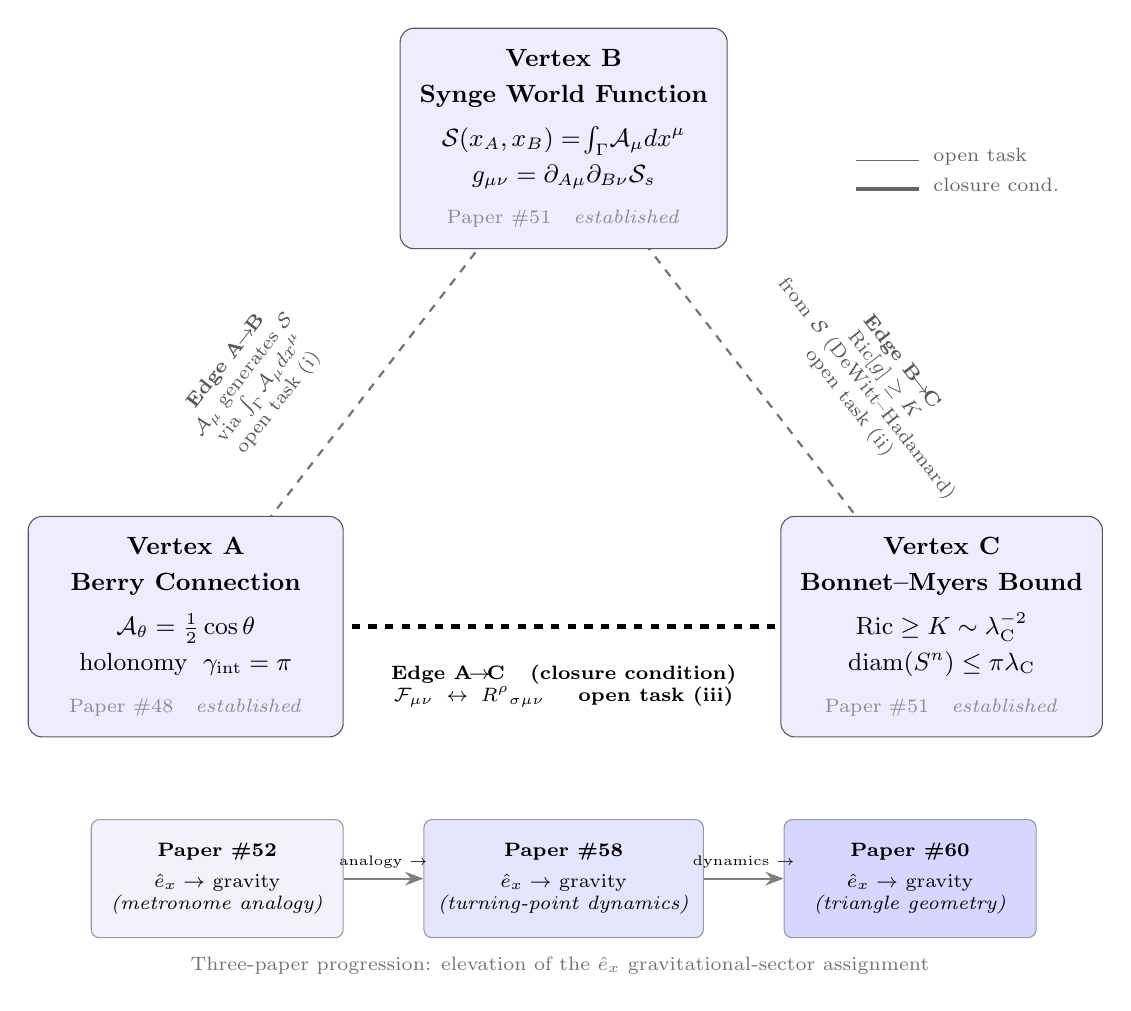
\begin{tikzpicture}[
  vtx/.style={
    rectangle, rounded corners=5pt,
    draw=black!65, fill=blue!7,
    minimum width=4.0cm, minimum height=2.8cm,
    align=center, font=\small, inner sep=7pt
  },
  openedge/.style={dashed, thick, draw=black!55, -Stealth},
  closureedge/.style={dashed, line width=1.8pt, draw=black, -Stealth},
  edgelbl/.style={font=\scriptsize, align=center, fill=white,
                  inner sep=2pt, draw=none, text=black!65},
  closurelbl/.style={font=\scriptsize\bfseries, align=center, fill=white,
                     inner sep=2pt, draw=none, text=black},
  stepbox/.style={rectangle, rounded corners=3pt,
                  draw=black!40, fill=gray!8,
                  minimum width=3.2cm, minimum height=1.5cm,
                  align=center, font=\scriptsize, inner sep=5pt},
  steparrow/.style={thick, draw=black!50, -Stealth},
]

% ── Vertex coordinates (equilateral-ish, scaled for column width) ──
\coordinate (A) at (0,   0);
\coordinate (B) at (4.8, 6.2);
\coordinate (C) at (9.6, 0);

% ── Edges (draw before nodes so nodes overlay arrow tips) ──
\draw[openedge]    (A) to (B);
\draw[openedge]    (B) to (C);
\draw[closureedge] (A) to (C);

% ── Edge labels ──
\node[edgelbl, rotate=52] at ($(A)!0.50!(B) + (-1.55, 0.0)$) {
  \textbf{Edge A$\!\to\!$B}\\
  $\mathcal{A}_\mu$ generates $\mathcal{S}$\\
  via $\int_\Gamma \mathcal{A}_\mu dx^\mu$\\
  open task~(i)
};

\node[edgelbl, rotate=-52] at ($(B)!0.50!(C) + (1.55, 0.0)$) {
  \textbf{Edge B$\!\to\!$C}\\
  $\mathrm{Ric}[g]\geq K$\\
  from $\mathcal{S}$ (DeWitt--Hadamard)\\
  open task~(ii)
};

\node[closurelbl] at ($(A)!0.50!(C) + (0, -0.75)$) {
  \textbf{Edge A$\!\to\!$C\quad(closure condition)}\quad \\
  $\mathcal{F}_{\mu\nu}\;\leftrightarrow\;R^\rho{}_{\sigma\mu\nu}$
  \quad open task~(iii)
};

% ── Vertex nodes ──
\node[vtx] at (A) {
  \textbf{Vertex A}\\[2pt]
  \textbf{Berry Connection}\\[5pt]
  $\mathcal{A}_\theta = \tfrac{1}{2}\cos\theta$\\[2pt]
  holonomy $\;\gamma_\mathrm{int} = \pi$\\[4pt]
  {\scriptsize\color{black!45}Paper~\#48\quad\emph{established}}
};

\node[vtx] at (B) {
  \textbf{Vertex B}\\[2pt]
  \textbf{Synge World Function}\\[5pt]
  $\mathcal{S}(x_A,x_B)=\!\int_\Gamma\!\mathcal{A}_\mu dx^\mu$\\[2pt]
  $g_{\mu\nu}=\partial_{A\mu}\partial_{B\nu}\mathcal{S}_s$\\[4pt]
  {\scriptsize\color{black!45}Paper~\#51\quad\emph{established}}
};

\node[vtx] at (C) {
  \textbf{Vertex C}\\[2pt]
  \textbf{Bonnet--Myers Bound}\\[5pt]
  $\mathrm{Ric}\geq K\sim\lambda_\mathrm{C}^{-2}$\\[2pt]
  $\mathrm{diam}(S^n)\leq\pi\lambda_\mathrm{C}$\\[4pt]
  {\scriptsize\color{black!45}Paper~\#51\quad\emph{established}}
};

% ── Legend (top-right) ──
\node[font=\scriptsize, align=left, text=black!60] at (9.8, 5.8) {
  \rule{0.8cm}{0.4pt}\ \ open task\\[3pt]
  \rule[0.5pt]{0.8cm}{1.2pt}\ \ closure cond.
};

% ── Three-paper progression inset (below triangle) ──
\node[stepbox, fill=blue!5] (S52) at (0.4, -3.2) {
  \textbf{Paper \#52}\\[3pt]
  $\hat{e}_x \to$ gravity\\
  \emph{(metronome analogy)}
};
\node[stepbox, fill=blue!10] (S58) at (4.8, -3.2) {
  \textbf{Paper \#58}\\[3pt]
  $\hat{e}_x \to$ gravity\\
  \emph{(turning-point dynamics)}
};
\node[stepbox, fill=blue!16] (S60) at (9.2, -3.2) {
  \textbf{Paper \#60}\\[3pt]
  $\hat{e}_x \to$ gravity\\
  \emph{(triangle geometry)}
};
\draw[steparrow] (S52) -- node[above, font=\tiny]{analogy $\to$} (S58);
\draw[steparrow] (S58) -- node[above, font=\tiny]{dynamics $\to$} (S60);

\node[font=\scriptsize, align=center, text=black!55] at (4.8, -4.3) {
  Three-paper progression: elevation of the $\hat{e}_x$ gravitational-sector assignment
};
\end{tikzpicture}
\end{figure*}


% ----------------------------------------
% Subsection A.3: The DeWitt-Hadamard Expansion
% ----------------------------------------
\subsection{The DeWitt--Hadamard Expansion}

For points $x$ and $x'$ close together, the Synge world function admits a Taylor expansion in the coordinate separation $y^\mu = (x-x')^\mu$~\cite{DeWitt1965,Hadamard1923}:
\begin{align}
\sigma(x,x') &= \frac{1}{2}g_{\mu\nu}\,y^\mu y^\nu
\notag\\
&\quad - \frac{1}{6}R_{\mu\nu\rho\sigma}\,y^\mu y^\nu y^\rho y^\sigma
\notag\\
&\quad + \frac{1}{20}\nabla_\alpha R_{\mu\nu\rho\sigma}\,y^\mu y^\nu y^\rho y^\sigma y^\alpha
\notag\\
&\quad + O(y^6),
\label{app:eq:dewitt}
\end{align}
where all curvature quantities are evaluated at $x$.
This expansion has two important features for the present paper.
First, the metric $g_{\mu\nu}$ appears at order $y^2$: the second derivative of $\sigma$ with respect to $y$ recovers the metric at leading order, consistent with the reconstruction theorem.
Second, the Riemann tensor $R_{\mu\nu\rho\sigma}$ appears at order $y^4$: the fourth derivative of $\sigma$ with respect to $y$ encodes the curvature.
This is why the DeWitt--Hadamard expansion is relevant for Edge~B$\to$C: if the 0-Sphere phase functional $\SyngeS$ admits an analogous expansion, its fourth-order coefficient would reveal whether the emergent metric has positive or negative curvature.

% ----------------------------------------
% Subsection A.4: The Van Vleck-Morette Determinant
% ----------------------------------------
\subsection{The Van Vleck--Morette Determinant}

The van Vleck--Morette determinant~\cite{VanVleck1928}:
\begin{equation}
\Delta(x,x') = \frac{-\det(-\nabla_{A\mu}\nabla_{B\nu}\,\sigma)}{\sqrt{g(x)\,g(x')}}
\label{app:eq:vvm}
\end{equation}
measures the ratio of the geodesic tube cross-sectional area at $x'$ to that at $x$.
In flat space, $\Delta = 1$.
In a positively curved space (Ricci curvature $> 0$), geodesics focus and $\Delta < 1$ for separated points; in a negatively curved space, geodesics defocus and $\Delta > 1$.
The Bonnet--Myers condition $\mathrm{Ric} \geq K > 0$ is therefore associated with $\Delta \leq 1$ and geodesic focusing, a signature that would appear in the short-distance behavior of the 0-Sphere phase functional $\SyngeS$ if Edge~B$\to$C is satisfied.

% ========================================
% Appendix B: Bonnet-Myers Theorem: Statement and Context
% ========================================
\section{Bonnet--Myers Theorem: Statement and Context}
\label{app:bonnet}

This appendix states the Bonnet--Myers theorem in the form used in this paper and explains its relevance to the compactness of the photon-sphere domain.

% ----------------------------------------
% Subsection B.1: Statement of the Theorem
% ----------------------------------------
\subsection{Statement of the Theorem}

Let $(M, g)$ be a complete Riemannian manifold of dimension $n \geq 2$.
Suppose that the Ricci curvature satisfies:
\begin{equation}
\mathrm{Ric}(v, v) \geq (n-1)\kappa\, g(v,v)
\label{app:eq:bonnet_condition}
\end{equation}
for all tangent vectors $v$ and some constant $\kappa > 0$.
Then~\cite{Myers1941,Chavel2006}:
\begin{enumerate}[label=(\alph*), leftmargin=1.5em]
\item The diameter of $M$ is bounded: $\mathrm{diam}(M) \leq \pi/\sqrt{\kappa}$.
\item $M$ is compact (bounded and complete).
\item The fundamental group $\pi_1(M)$ is finite.
\end{enumerate}
In the 0-Sphere Model, the Ricci curvature of the photon sphere is assumed to satisfy $\mathrm{Ric} \geq K$ with $K \sim \lambdaC^{-2}$, so $\kappa = K/( n-1) \sim \lambdaC^{-2}/(n-1)$ and the bound becomes $\mathrm{diam} \leq \pi\lambdaC\sqrt{n-1}$, which reduces to $\pi\lambdaC$ for $n = 2$ (the photon sphere surface).

% ----------------------------------------
% Subsection B.2: Relevance to the Triangle
% ----------------------------------------
\subsection{Relevance to the Triangle}

The Bonnet--Myers theorem connects Vertex~B (metric curvature) to Vertex~C (compact domain) through Edge~B$\to$C.
If the emergent metric $g_{\mu\nu} = \partial_{A\mu}\partial_{B\nu}\SyngeS_s$ has positive Ricci curvature $K \sim \lambdaC^{-2}$, then the Bonnet--Myers theorem guarantees the compactness of the photon sphere domain and the finiteness of its fundamental group $\pi_1$.
The finite $\pi_1$ has a direct consequence for the Berry connection of Vertex~A: holonomies of U(1) connections over a compact base with finite $\pi_1$ take values in a discrete subgroup of U(1), which is the structural reason why $\gamma_\mathrm{intrinsic} = \pi$ is topologically protected rather than continuously deformable.
This link between Vertex~B, Vertex~C, and Vertex~A is the content of Edge~A$\to$C and is the reason the triangle is a triangle rather than three disconnected conditions.

% ========================================
% Appendix C: The Triangle Diagram and the Three-Paper Progression
% ========================================
\section{The Triangle Diagram and the Three-Paper Progression}
\label{app:triangle_figure}

This appendix provides a visual summary of the Berry--Synge--Bonnet--Myers triangle (Fig.~\ref{fig:triangle_full}) and a self-contained account of the three-paper progression (\#52 $\to$ \#58 $\to$ \#60) that led to its formulation.
The figure is designed for readers who approach the series non-linearly and need a single-diagram orientation.

% ----------------------------------------
% Subsection C.1: The Geometric Triangle
% ----------------------------------------
\subsection{The Geometric Triangle}

Figure~\ref{fig:triangle_full} displays the three established vertices and three open edges of the triangle.
Filled rectangular boxes represent the three vertices, each an established result.
Dashed arrows represent the three edges, each an open structural condition.
The bottom edge (Edge~A$\to$C, thick dashed) is the closure condition: if satisfied, Berry curvature $\BerryF_{\mu\nu}$ and the Riemann tensor $R^\rho{}_{\sigma\mu\nu}$ are identified on the Bonnet--Myers-bounded compact domain, unifying the gauge and gravitational sectors from a single phase functional $\SyngeS(x_A, x_B)$.

% ----------------------------------------
% Subsection C.2: The Three-Paper Progression: e_x from Analogy to Geometry
% ----------------------------------------
\subsection{The Three-Paper Progression: $\ehat{x}$ from Analogy to Geometry}
\label{app:three_paper}

The gravitational-sector assignment $\ehat{x} \to \text{gravity}$ was introduced, elevated, and geometrically grounded across three consecutive papers in the series.
This subsection provides a self-contained account for readers who encounter the assignment for the first time in the present paper.

\paragraph{Stage 1: Metronome analogy (Paper \#52~\cite{hanamura52}).}
Paper~\#52 established the $\lambda_\mathrm{C}$ cancellation theorem (Theorem 2.1 of that paper): the Compton wavelength cancels exactly from the gravitational force formula because the ZB axis $\hat{e}$ governs both the energy-collection lever arm (Role~I: $\delta E \propto \lambda_\mathrm{C}(\hat{e}\cdot\hat{g})$) and the ZB cycle rate (Role~II: $\omega_\mathrm{ZB}/2\pi = \vZB/\lambda_\mathrm{C}$), both sharing the same geometric origin.
The resulting force $F = m_e g \betaZB$ is independent of particle mass, constituting a structural derivation of the weak equivalence principle.
The assignment $\ehat{x} \to \text{gravity}$ in Paper~\#52 rested on the metronome analogy: gravitational coupling, like metronome synchronization, operates \emph{parallel} to the oscillation direction, while electromagnetic coupling (Larmor radiation) operates transversely, like a Yagi--Uda antenna.
This assignment was structural and physically motivated, but analogy-based.

\paragraph{Stage 2: Turning-point dynamics (Paper \#58~\cite{hanamura58}).}
Paper~\#58 resolved open task~(vi) of Paper~\#49 by identifying the spin-2 character of the gravitational mediator with the phase-stable pair of photon-sphere ejection events.
The key observation was that the Thomas angular velocity $\OmT(\iphase) \propto \sin(2\iphase)$ has period $\pi$ (half the ZB period), so its magnitude reaches its maximum at \emph{two} points per ZB cycle: $\iphase_1 = \pi/2$ and $\iphase_2 = 3\pi/2$.
At both points, the $\ehat{x}$ component of the photon-sphere velocity vanishes: $\dot{x}(\iphase) = \vZB\cos\iphase = 0$.
The ejection events occur precisely where the photon sphere momentarily stops along the propagation axis.
This is the dynamical reason why $\ehat{x}$ is the emission direction for the spin-2 gravitational mediator: it is not merely the direction that is parallel to the oscillation (analogy), but the direction along which the oscillation comes to rest at the moment of maximal Thomas-precession stress (mechanical fact).
The combined polarization tensor of the two ejection events is $h_{\mu\nu} \propto \varepsilon_{1\mu}\varepsilon_{2\nu} + \varepsilon_{1\nu}\varepsilon_{2\mu}$, a rank-2 symmetric object carrying helicity $\pm 2$.

\paragraph{Stage 3: Geometric conditions (Paper \#60, the present paper).}
The present paper formulates the geometric basis for the $\ehat{x}$ assignment by identifying the Berry--Synge--Bonnet--Myers triangle as the framework within which $\ehat{x}$ acquires its role.
The Berry connection $\BerryA_\mu$ is a spacetime 1-form whose integration along $\Gamma_\mathrm{ext}$ (the helical arc propagating along $\ehat{x}$) generates the phase functional $\SyngeS(x_A,x_B)$.
This functional, identified as the Synge world function, yields the metric $g_{\mu\nu} = \partial_{A\mu}\partial_{B\nu}\SyngeS_s$ through the Synge reconstruction theorem.
The Berry curvature $\BerryF_{\mu\nu} = \partial_\mu\BerryA_\nu - \partial_\nu\BerryA_\mu$ of the same connection, when identified with the Riemann tensor $R^\rho{}_{\sigma\mu\nu}$ of this metric on the Bonnet--Myers compact domain (Edge~A$\to$C, the closure condition), establishes that the direction of integration --- $\ehat{x}$ --- is simultaneously the direction of gravitational phase accumulation and the direction in which the Berry curvature corresponds to spacetime curvature.
\textbf{The closure of the triangle} (Edge~A$\to$C) is the geometric statement that the $\ehat{x}$ gravitational-sector assignment is not analogical or merely dynamical, but a necessary consequence of the internal geometry of the phase accumulation functional.

The three stages are not merely rhetorical.
Each stage adds a layer of necessity.
Analogy makes the assignment plausible.
Dynamics makes it mechanically inevitable (the turning-point structure forces $\ehat{x}$).
Geometry makes it logically necessary (closing the triangle would mean there is no other consistent assignment for the gravitational sector in the 0-Sphere framework).

\clearpage

% ========================================
% End of Document
% ========================================
\end{document}